%        File: main.tex
%     Created: Tue Sep 13 12:00 PM 2022 M
% Last Change: Tue Sep 13 12:00 PM 2022 M
%
\documentclass[a4paper]{article}
\usepackage[utf8]{inputenc}

\title{Assignment 2}
\author{lamsonbrady }
\date{September 3rd, 2022}

% General packages
\usepackage{parskip}

% Header related stuff
\usepackage{fancyhdr}
\pagestyle{fancy}
\fancyhead[R]{MTH 3220 - Linear Algebra}  
\fancyhead[L]{Homework 2}               
\fancyfoot[R]{Brady Lamson}
\fancyfoot[L]{MSU Denver}

% Math packages
\usepackage{amsmath}
\usepackage{amssymb}

% Creates small p-matrix ----
\newcommand{\psmall}[1]{
\left(\begin{smallmatrix}
#1
\end{smallmatrix} \right)
}

% makes mathbb commands faster to type
\newcommand{\bb}{\mathbb}

% Makes vectors slightly faster
% \newcommand{\v}[#1]{\vec{#1}}

\begin{document}
\part*{Linear Transformations}

\section{Question 1}
How do we find the matrix of a linear transformation?

\subsection{Example 1}

\[
T:\R^2 \to \R^2 \\
\]

$T(\vec{v}) = $ symmetric image over the x-axis

Note: Think of a vector going to $\psmall{1\\1}$ flipping over the x-axis and now being $\psmall{1\\-1}$

In terms of generic coordinates we have this transformation

\[
	\begin{aligned}
		T(\vec{v}) &= \genericmat{p}{a_1\\-a_2} = \genericmat{p}{1&0\\0&-1} \cdot \genericmat{p}{a_1\\a_2} \\
		T\genericmat{p}{a_1\\a_2} &= \genericmat{p}{a_1-a_2\\2a_1+3a_2}
	\end{aligned}
\]

\subsection{Example 2}

\[T:\R^2 \to \R^2\]

That reflects the vector over $x_1 = x_2$

\[
	\begin{aligned}
		T(\vec{e_1}) &= \vec{e_2} = \genericmat{p}{0\\1} \\
		T(\vec{e_2}) &= \vec{e_1} = \genericmat{p}{1\\0} \\
	\end{aligned}
\]

So our matrix is $A_T = \genericmat{p}{0&1\\1&0}$

\section*{Proposition}
This is the theorem initially brought up in week 3 notes.

A transformation is linear IF AND ONLY IF there exists an $m \times n$ matrix A such that $\boxed{T(\vec{v}) = A_t\vec{v}}$

Note: In the same way a quadratic function may make the math student visualize a parabola, let linear transformations make matrix multiplication come to mind.

\subsection{Proof}

First: $P \to Q$

Let $\vec{v} \in \R^n$ be a domain vector, so we can write 

\[
	\vec{v} = \genericmat{p}{a_1\\a_2\\ \dots\\a_n} = a_1 \vec{e_1} + a_2 \vec{e_2} + \dots + a_n \vec{e_n}
\]

Then 

\[
	T(\vec{v}) = T(a_1 \vec{e_1} + a_2 \vec{e_2} + \dots + a_n \vec{e_n})
\]

And, because $T(\vec{v_1} + \vec{v_2}) = T(\vec{v_1}) + T(\vec{v_2})$

\[
	T(\vec{v}) = T(a_1 \vec{e_1}) + T(a_2 \vec{e_2}) + \dots + a_n \vec{e_n}
\]

And, because $T(\alpha \vec{v}) = \alpha T(\vec{v})$

\[
	\begin{aligned}
		T(\vec{v}) &= a_1T(\vec{e_1}) + a_2T(\vec{e_2}) + \dots + a_nT(\vec{e_n}) \\
		T\genericmat{p}{a_1\\a_2\\ \dots \\a_n} &= \genericmat{p}{T(e_1) & T(e_2) & \dots & T(e_n)} \cdot \genericmat{p}{a_1\\a_2\\ \dots \\ a_n}
	\end{aligned}
\]

\subsection{Example 3 (Vectors)}

\[
T: \R^2 \to \R^2
\]

$T(\vec{v})$ is the rotation of $\vec{v}$ by an angle $\gamma$.

\[
	\begin{aligned}
		T\genericmat{p}{a_1\\a_2} = \genericmat{p}{? & ? \\ ? & ?} \cdot \genericmat{p}{a_1\\a_2}
	\end{aligned}
\]

Picture a triangle with radius 1. So we have length = 1, x coordinate $cos(\gamma)$, y coordinate $sin(\gamma)$. This is a basic triangle, probably around 45 degrees.

Now picture a triangle with radius 1, except we're now in quadrant 2. The flat top of the triangle extends out of the y-axis. Imagine $\gamma \approx 135$ degrees. So now we have length 1, x coordinate is $-sin(\gamma)$, y coordinate of $cos(\gamma)$. 

Something roughly like this! 

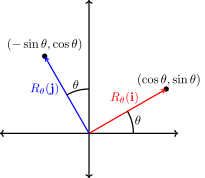
\includegraphics[scale=0.75]{fig1}

\[
	\begin{aligned}
		T\genericmat{p}{a_1\\a_2} &= \genericmat{p}{cos(\gamma) & -sin(\gamma)\\sin(\gamma) & cos(\gamma)} \cdot \genericmat{p}{a_1\\a_2}
		\\
		&= \genericmat{p}{a_1 cos(\gamma) - a_2 sin(\gamma) \\ a_1 sin(\gamma) + a_2 cos(\gamma)}
	\end{aligned}
\]

\subsection{Example 4 (Matrices)}

\[
	\begin{aligned}
		T: M_{2 \times 2}(\R) \to \R \\
		T(A) = \text{Trace}(A)
	\end{aligned}
\]

\subsubsection{Definition}
Given a matrix A, we define the Trace(A) as the sum of all diagonal entries. 

\[\text{trace}(A) = \sum_{i=1}^{n}a_{ii}\]

So,

\[
	T \genericmat{p}{a&b\\c&d} = a + d
\]

Basis for $M_{2 \times 2}$ is $E_{11}, E_{12}, E_{21}, E_{22}$. The basis for $\R$ is just $1$.

From this, we should end up with a $1 \times 4$ matrix! Ask yourself why.

These 4 columns will be $T(E_{11}),T(E_{12}),T(E_{21}),T(E_{22})$

Going through the traces for each of these:

\[
	\begin{aligned}
		T(E_{11}) &= \text{trace}\genericmat{p}{1 & 0\\0&0} = 1 \\
		T(E_{12}) &= \text{trace}\genericmat{p}{0 & 1\\0&0} = 0 \\
		T(E_{21}) &= \text{trace}\genericmat{p}{0 & 0\\1&0} = 0 \\
		T(E_{22}) &= \text{trace}\genericmat{p}{0 & 0\\0&1} = 1
	\end{aligned}
\]

So 

\[
	A_T = (1,0,0,1)
\]

From this,

\[T(\vec{v}) = A_T \vec{v}\]

\[T \genericmat{p}{a&b\\c&d} = (1 0 0 1) \cdot \genericmat{p}{a\\b\\c\\d}\]

\[T \genericmat{p}{a&b\\c&d} = a + 0 + 0 + d = a + d\]

\subsection{Example 5 (Polynomials)}
\[T: \P_3 \to \P_2\]
\[T(p(t)) = \frac{dp}{dt}\]

The derivative transform.

$\P_3$ has basis $\left\{ 1, t, t^2, t^3 \right\}$

$\P_2$ has basis $\left\{ 1, t, t^2 \right\}$

My matrix then is a $3 \times 4$ matrix with columns T(1), T(t), $T(t^2)$, $T(T^3)$.

\subsubsection{Side note}
We change polynomial vectors with their coordinate vectors.

Example: $\vec{v} = 2 - t + t^3 \to \genericmat{p}{2 \\ -1 \\ 0 \\ 1}$

Resuming,

Let us list out our transformations and their coordinates

\[
	\begin{aligned}
		1 \to T(1) = 0 \to \genericmat{p}{0\\0\\0} \\
		t \to T(t) = 1 \to \genericmat{p}{1\\0\\0} \\
		t^2 \to T(t^2) = 2t \to \genericmat{p}{0\\2\\0} \\
		t^3 \to T(t^3) = 3t^2 \to \genericmat{p}{0\\0\\3} \\
	\end{aligned}
\]

So my matrix is 

\[A_T = \genericmat{p}{0&1&0&0 \\ 0&0&2&0 \\ 0&0&0&3}\]

\part{Thursday Notes}

Vector spaces lead to the basis of a vector space. Within this space we have a relationship between theoretical vectors and euclidean vectors.

\[
	\vec{v} = x_1 \vec{v_1} + x_2 \vec{v_2} + \dots + x_n \vec{v_n} 
	\longleftrightarrow
	\vec{v} = \genericmat{p}{x_1\\x_2\\ \vdots \\ x_n}
\]

And, also building off of the basis of a vector space are linear transformations. These have the same kind of relationship between theoretical transformations and matrix representations.

\[
	\begin{aligned}
	T(\vec{v_1} + \vec{v_2}) = T\left( \vec{v_1} \right)) + T\left( \vec{v_2} \right)
	\longleftrightarrow
	T(\vec{v}) = A_T \cdot \vec{v}
	\end{aligned}
\]

\section{Matrices and Systems of Linear Equations}
\subsection{Question 1}

Consider the vectors

\[
	\vec{v_1} = \genericmat{p}{1\\-2\\3} \genericmat{p}{1\\-1\\2} \genericmat{p}{2\\-3\\6}
\]

\subsubsection{A}

Show that $\vec{v_1}, \vec{v_2}, \vec{v_3}$ are linearly independent.

\subsubsection{B}

Write the vector $\vec{b} = \psmall{6\\5\\4}$ as a linear combination of $\{\vec{v_1}, \vec{v_2}, \vec{v_3}\}$

\subsubsection{C}

Explain, using the basis definition, why $\{\vec{v_1}, \vec{v_2}, \vec{v_3}\}$ form a basis for $\R^3$

\end{document}


